%!TEX root = ./template-skripsi.tex

\subsection{Sprint 4 Report}
Berikut merupakan report dari sprint ke-4 yang dilakukan pada tanggal 15 juni - 21 juni 2022.

\begin{table}[H]
	\caption{\textit{Sprint-4 backlog}}
	\label{sprint4_backlog}
	\begin{tabular}{@{} |p{0.5cm}|p{5cm}|p{5cm}|p{2cm}| @{}}
		\hline
		\textbf{No} & \textbf{\textit{Story}} & \textbf{\textit{Task}} & \textbf{\textit{Status}} \\
		\hline
		1 & \multirow{3}{5cm}{Create, Read, Updte, dan Delete untuk Masa Budidaya Kolam} & Membarui desain database  & Completed\\
		\cline{1-1}\cline{3-4}
		2 & & Implementasi API aktifasi kolam & Completed\\
		\cline{1-1}\cline{3-4}
		3 & & Implementasi API deaktifasi kolam & Completed\\
		\cline{1-1}\cline{3-4}
		4 & & Implementasi API fetch list status kolam & Completed\\
		\cline{1-1}\cline{3-4}
		5 & & Implementasi API fetch musim budidaya per kolam & Completed\\
		\cline{1-1}\cline{3-4}
		6 & & Membuat view status budidaya semua kolam & Completed\\
		\cline{1-1}\cline{3-4}
		7 & & Membuat view list budidaya per kolam & Completed\\
		\cline{1-1}\cline{3-4}
		8 & & Membuat view detail budidaya & Completed\\
		\cline{1-1}\cline{3-4}
		\hline
	\end{tabular}
\end{table}

\begin{enumerate}[1.]



\item \textbf{Membarui desain database}

\begin{figure}[H]
	\centering
	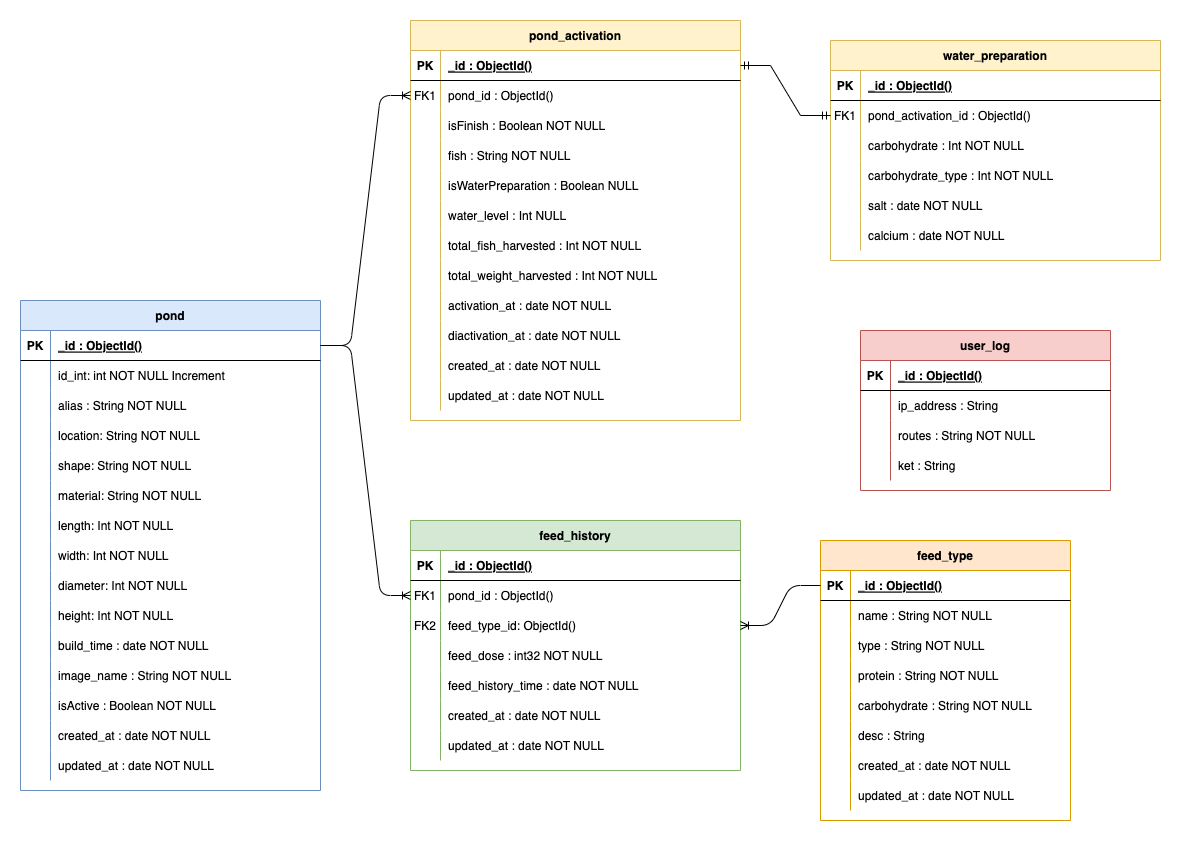
\includegraphics[height=0.7\textwidth]{gambar/Sprint04/diagram database/database}
	\caption{ERD Database Sprint-4}
	\label{fig:database_sprint4}
\end{figure}

Dengan berubahnya desain database diperlukan juga penambahan model pada source code, berikut perubahan pada source code model.

\begin{lstlisting}
# fishapi/database/model.py

class PondActivation(db.Document):
    id_int = db.IntField(required=True)
    pond_id = db.ReferenceField(Pond, required=True)
    isFinish = db.BooleanField(required=True, default=False)
    isWaterPreparation = db.BooleanField(required=True, default=False)
    water_level = db.FloatField(required=True, default=0)
    total_fish_harvested = db.IntField(required=True, default=0)
    total_weight_harvested = db.IntField(required=True, default=0)
    activated_at = db.DateTimeField(default=datetime.datetime.now)
    deactivated_at = db.DateTimeField(default=None)
    deactivated_description = db.StringField(default=None)
    constanta_oversize = db.FloatField(required=True, default=1.3)
    constanta_undersize = db.FloatField(required=True, default=0.7)
    created_at = db.DateTimeField(default=datetime.datetime.now)
    updated_at = db.DateTimeField(default=datetime.datetime.now)
\end{lstlisting}



\item \textbf{Implementasi API aktifasi kolam}

Perubahan terjadi pada controller API entry musim budidaya, berikut merupakan perubahan source code controller API entry musim budidaya.

\begin{lstlisting}
# fishapi/database/pondactivation.py

class PondActivationApi(Resource):
    def post(self, pond_id):
        pond = Pond.objects.get(id=pond_id)
        pipeline_year = {'$match': {'$expr': {'$and': [
                        {'$eq': ['$pond_id', {'$toObjectId': pond_id}]},
                        {'$eq': [{'$dateToString': {
                            'format': "%Y", 'date': "$created_at"}}, getYearToday()]},
        ]
        }}}
        list_pond_year = PondActivation.objects.aggregate(pipeline_year)
        list_pond_year = list(list_pond_year)
        id_int = len(list_pond_year) + 1
        if pond.isActive == True:
            response = {"message": "status pond is already active"}
            response = json.dumps(response, default=str)
            return Response(response, mimetype="application/json", status=400)
        fishes = request.form.get("fish", "[]")
        fishes = json.loads(fishes)
        if len(fishes) < 1:
            response = {"message": "There is no fish"}
            response = json.dumps(response, default=str)
            return Response(response, mimetype="application/json", status=400)
        isWaterPreparation = request.form.get("isWaterPreparation", False)
        if isWaterPreparation == "true":
            isWaterPreparation = True
        else:
            isWaterPreparation = False
        water_level = request.form.get("water_level", None)
        activated_at = request.form.get(
            "activated_at", datetime.datetime.now())
        pond_activation_data = {
            "id_int": id_int,
            "pond_id": pond_id,
            "isFinish": False,
            "isWaterPreparation": isWaterPreparation,
            "water_level": water_level,
            "activated_at": activated_at
        }
        pondActivation = PondActivation(**pond_activation_data).save()
        pondActivation_id = pondActivation.id
        if isWaterPreparation == True:
            carbohydrate = request.form.get("carbohydrate", None)
            carbohydrate_type = request.form.get("carbohydrate_type", None)
            salt = request.form.get("salt", None)
            calcium = request.form.get("calcium", None)
            water_preparation_data = {
                "pond_activation_id": pondActivation_id,
                "carbohydrate": carbohydrate,
                "carbohydrate_type": carbohydrate_type,
                "salt": salt,
                "calcium": calcium,
            }
            water_preparation = WaterPreparation(
                **water_preparation_data).save()
        pond.update(**{"isActive": True})
        for fish in fishes:
            # save fish log
            data = {
                "pond_id": pond_id,
                "pond_activation_id": pondActivation_id,
                "type_log": "activation",
                "fish_type": fish['type'],
                "fish_amount": fish['amount'],
                "fish_total_weight": fish['weight']
            }
            fishlog = FishLog(**data).save()
        response = {"message": "success to activation pond"}
        response = json.dumps(response, default=str)
        return Response(response, mimetype="application/json", status=200)
\end{lstlisting}

Kode tersebut adalah sebuah fungsi dalam sebuah REST API yang bertujuan untuk mengaktifkan kolam ikan. Pada awal fungsi, dilakukan pencarian kolam ikan berdasarkan id kolam yang diberikan.

Selanjutnya, dilakukan operasi agregasi MongoDB untuk mencari data aktivasi pada tahun ini dengan menggunakan metode \$match dan memanfaatkan fungsi agregasi lainnya seperti \$and, \$eq, \$dateToString, dan getYearToday(). Hasil agregasi kemudian disimpan dalam variabel list\_pond\_year.

Selanjutnya, variabel id\_int dihitung berdasarkan panjang dari list\_pond\_year ditambah 1. Kemudian, dilakukan beberapa validasi seperti memeriksa apakah kolam sudah aktif atau belum, dan apakah terdapat ikan yang akan dimasukkan ke dalam kolam.

Jika semua validasi telah dilakukan, data aktivasi kolam akan disimpan dalam database, lalu dilakukan pembaruan pada status kolam menjadi aktif. Data ikan yang dimasukkan ke dalam kolam juga akan disimpan dalam bentuk log pada tabel FishLog.

Terakhir, fungsi mengembalikan respons dalam format JSON yang berisi pesan berhasil atau gagalnya aktivasi kolam.

Berikut merupakan form untuk entry musim budidaya.

\begin{longtable}{| l | p{5cm} | p{5cm} |}
\caption{Form entry musim budidaya kolam.\label{table:form_entry_musim_budidaya}}\\

\hline
\multicolumn{1}{|c|}{\textbf{Form}} & \multicolumn{1}{|c|}{\textbf{Jenis Data}} & \multicolumn{1}{|c|}{\textbf{Deskripsi}}\\
\hline
\endfirsthead

\hline
\multicolumn{3}{|c|}{Lanjutan Tabel \ref{table:form_entry_musim_budidaya}}\\
\hline
\multicolumn{1}{|c|}{\textbf{Form}} & \multicolumn{1}{|c|}{\textbf{Jenis Data}} & \multicolumn{1}{|c|}{\textbf{Deskripsi}}\\
\hline
\endhead

                                          
fish               & REQUIRED STRING FORMAT list(dict()) jenis ikan : {[}"nila merah", "nila hitam", "lele", "patin", "mas"{]} ex: "{[}\{"lele": 100\},\{"patin":200\}{]}" & jenis ikan dan jumlah ikan                             \\ \hline
isWaterPreparation & REQUIRED STRING BOOLEAN                                                                                                                               & variable bila aktifasi kolam menggunakan preparasi air \\ \hline
water\_level       & REQUIRED DOUBLE                                                                                                                                       & ketinggian air dalam meter (m)                         \\ \hline
activated\_at      & OPTIONAL STRING DATE FORMAT : isodate()                                                                                                               & timestamp aktifasi kolam                               \\ \hline
carbohydrate       & REQUIRED INTEGER IF isWaterPreparation == True                                                                                                        & banyak karbohidrat dalam (Gram/ml)                     \\ \hline
carbohydrate\_type & REQUIRED STRING IF isWaterPreparation == True VALUE : {[}"gula", "molase", "trigu", "tapioka",{]}                                                     & jenis karbohidrat yang di gunakan                      \\ \hline
salt               & REQUIRED INTEGER IF isWaterPreparation == True                                                                                                        & berat garam yang di gunakan (Kg)                       \\ \hline
calcium            & REQUIRED INTEGER IF isWaterPreparation == True                                                                                                        & berat kapur yang di gunakan (gram)                     \\ \hline

\end{longtable}


Tabel di atas berisi informasi tentang parameter yang harus diisi atau opsional dalam aktivasi atau memulai musim budidaya kolam ikan. Berikut adalah penjelasan masing-masing kolom pada tabel tersebut:

\begin{enumerate}
\item Form: Merupakan nama parameter yang harus diisi atau opsional dalam aktivasi kolam ikan.
\item Jenis Data: Menjelaskan jenis data yang harus diisi pada parameter tersebut. Contohnya, string, boolean, integer, atau double.
\item Deskripsi: Berisi deskripsi singkat tentang informasi yang harus diisi pada parameter tersebut.
\end{enumerate}

Beberapa contoh parameter yang harus diisi pada aktivasi kolam ikan di antaranya adalah jenis ikan dan jumlahnya, ketinggian air dalam meter, dan variable bila aktivasi kolam menggunakan preparasi air. Ada juga parameter yang opsional, seperti timestamp aktifasi kolam. Selain itu, ada parameter yang harus diisi jika variable bila aktivasi kolam menggunakan preparasi air diaktifkan, seperti banyak karbohidrat dalam gram/ml dan jenis karbohidrat yang digunakan. Ada juga parameter yang harus diisi jika menggunakan kapur atau garam dalam preparasi air, yaitu berat kapur dan berat garam yang digunakan. Semua parameter ini harus diisi dengan format yang sudah ditentukan pada kolom Jenis Data.

Berikut merupakan hasil test request dari API aktivasi kolam.

cURL:

\begin{lstlisting}
curl --location -g 'http://jft.web.id/fishapi/api/ponds/{pond_id}/activation' \
--form 'fish="[{\"lele\": 100},{\"patin\":200}]"' \
--form 'isWaterPreparation="false"' \
--form 'water_level="100"'
\end{lstlisting}

response json:

\begin{lstlisting}
{
  "message": "success to activation pond"
}
\end{lstlisting}



\item \textbf{Implementasi API deaktifasi kolam}

Penambahan terjadi pada controller API entry musim budidaya, berikut merupakan perubahan source code controller API entry panen musim budidaya.

\begin{lstlisting}
# fishapi/database/pondactivation.py

class PondDeactivationApi(Resource):
    def post(self, pond_id):
        pond = Pond.objects.get(id=pond_id)
        if pond.isActive == False:
            response = {"message": "status pond is already not active"}
            response = json.dumps(response, default=str)
            return Response(response, mimetype="application/json", status=400)
        # get last pond_activation
        pond_activation = PondActivation.objects(
            pond_id=pond_id, isFinish=False).order_by('-activated_at').first()
        fishes = request.form.get("fish", "[]")
        fishes = json.loads(fishes)
        total_fish_harvested = 0
        total_weight_harvested = 0
        for fish in fishes:
            # save fish log
            data = {
                "pond_id": pond_id,
                "pond_activation_id": pond_activation.id,
                "type_log": "deactivation",
                "fish_type": fish['type'],
                "fish_amount": fish['amount'],
                "fish_total_weight": fish['weight']
            }
            total_fish_harvested += fish['amount']
            total_weight_harvested += fish['weight']
            fishlog = FishLog(**data).save()
            print(data)
        print(total_fish_harvested)
        print(total_weight_harvested)
        # get args form data
        # update pond_activation
        pond_deactivation_data = {
            "isFinish": True,
            "total_fish_harvested": total_fish_harvested,
            "total_weight_harvested": total_weight_harvested,
            "deactivated_at": request.form.get("deactivated_at", datetime.datetime.now()),
            "deactivated_description": "Normal"
        }
        pond_activation.update(**pond_deactivation_data)
        # update pond isActive
        pond.update(**{"isActive": False})
        response = {"message": "success to deactivation pond"}
        response = json.dumps(response, default=str)
        return Response(response, mimetype="application/json", status=200)
\end{lstlisting}

Kode ini merupakan sebuah kelas Python dengan nama PondDeactivationApi yang diturunkan dari kelas Resource. Kelas ini memiliki satu method yaitu post() yang mengambil satu argumen yaitu pond\_id.

Dalam method post(), dilakukan pengambilan data Pond dengan id tertentu yang diberikan sebagai argumen. Kemudian, jika atribut isActive pada objek Pond bernilai False, maka akan dikembalikan respons dengan pesan "status pond is already not active" dan status kode 400.

Selanjutnya, dilakukan pengambilan PondActivation terakhir yang memiliki pond\_id tertentu dan isFinish bernilai False. Kemudian, dilakukan pengolahan data ikan dengan mengambil nilai dari form data "fish", yang kemudian di-parse dari string JSON menjadi list Python. Dalam loop for, dilakukan penyimpanan data FishLog untuk setiap ikan yang terdapat dalam list fishes.

Setelah itu, dilakukan pembaruan data pada objek PondActivation dengan mengubah nilai atribut isFinish menjadi True dan menambahkan data mengenai total jumlah ikan yang dipanen (total\_fish\_harvested) dan total berat ikan yang dipanen (total\_weight\_harvested), serta waktu dan deskripsi pada saat deaktivasi. Selanjutnya, dilakukan pembaruan data pada objek Pond dengan mengubah nilai atribut isActive menjadi False.

Akhirnya, dilakukan pembuatan respons dengan pesan "success to deactivation pond" dan status kode 200. Pesan respons dan data lainnya kemudian di-serialize menjadi string JSON dengan menggunakan modul json dan dikembalikan dalam bentuk response dengan tipe konten "application/json".

Berikut merupakan form untuk entry panen musim budidaya.

\begin{longtable}{| l | p{5cm} | p{5cm} |}
\caption{Form entry panen musim budidaya kolam.\label{table:form_entry_panen_musim_budidaya}}\\

\hline
\multicolumn{1}{|c|}{\textbf{Form}} & \multicolumn{1}{|c|}{\textbf{Jenis Data}} & \multicolumn{1}{|c|}{\textbf{Deskripsi}}\\
\hline
\endfirsthead

\hline
\multicolumn{3}{|c|}{Lanjutan Tabel \ref{table:form_entry_musim_budidaya}}\\
\hline
\multicolumn{1}{|c|}{\textbf{Form}} & \multicolumn{1}{|c|}{\textbf{Jenis Data}} & \multicolumn{1}{|c|}{\textbf{Deskripsi}}\\
\hline
\endhead


total\_fish\_harvested   & REQUIRED INTEGER                                        & banyak ikan yang di angkat        \\ \hline
total\_weight\_harvested & REQUIRED INTEGER                                        & berat seluruh ikan yang di angkat \\ \hline
diactived\_at            & OPTIONAL STRING DATE FORMAT : isodate() DEFAULT : now() & timestamp diaktifasi kolam        \\ \hline

\end{longtable}

Tabel ini terdiri dari 3 baris, dimana setiap baris merepresentasikan sebuah parameter yang dapat digunakan dalam suatu API. Setiap baris terdiri dari 3 kolom yaitu:

\begin{enumerate}
\item Form : Merupakan nama parameter yang digunakan dalam API.
\item Jenis Data : Menjelaskan jenis data yang diterima oleh parameter tersebut. Pada tabel ini, Jenis Data terdiri dari REQUIRED INTEGER dan OPTIONAL STRING DATE FORMAT : isodate() DEFAULT : now().
\begin{enumerate}
\item REQUIRED INTEGER artinya bahwa parameter tersebut wajib diisi dengan nilai berupa bilangan bulat (integer).
\item OPTIONAL STRING DATE FORMAT : isodate() DEFAULT : now() artinya bahwa parameter tersebut bersifat opsional dan dapat diisi dengan nilai berupa string yang merepresentasikan tanggal dan waktu dalam format ISO (isodate), dengan nilai default saat tidak diisi adalah waktu saat ini.
\end{enumerate}
\item Deskripsi : Menjelaskan secara singkat tentang parameter tersebut. Pada tabel ini, Deskripsi menjelaskan tentang banyak ikan yang diangkat, berat seluruh ikan yang diangkat, dan timestamp diaktifasi kolam.
\end{enumerate}

Berikut merupakan hasil test request dari API deaktifasi/panen masa budidaya kolam.

cURL:
\begin{lstlisting}
curl --location -g 'http://jft.web.id/fishapi/api/ponds/{pond_id}/diactivation' \
--form 'total_fish_harvested="300"' \
--form 'total_weight_harvested="3000"'
\end{lstlisting}

response json:
\begin{lstlisting}
{
  "message": "success to diactivation pond"
}
\end{lstlisting}



\item \textbf{Implementasi API fetch list status kolam}

Penambahan terjadi pada controller API fetch list status kolam, berikut merupakan perubahan source code controller API fetch list status kolam.

\begin{lstlisting}
# fishapi/database/pondactivation.py

class PondsStatusApi(Resource):
    def get(self):
        pipline = [
            {'$lookup': {
                'from': 'pond_activation',
                'let': {"pondid": "$_id"},
                'pipeline': [
                    {'$match': {'$expr': {'$and': [
                        {'$eq': ['$pond_id', '$$pondid']},
                    ]}}},
                    {'$lookup': {
                        'from': 'water_preparation',
                        'let': {"pond_activation_id": "$_id"},
                        'pipeline': [
                            {'$match': {
                                '$expr': {'$eq': ['$pond_activation_id', '$$pond_activation_id']}}},
                            {"$project": {
                                "created_at": 0,
                                "updated_at": 0,
                            }}
                        ],
                        'as': 'water_preparation'
                    }},
                    {"$addFields": {
                        "water_preparation": {"$first": "$water_preparation"}
                    }},
                    {"$project": {
                        "pond_id": 0,
                        "feed_type_id": 0,
                        "created_at": 0,
                        "updated_at": 0,
                    }}
                ],
                'as': 'pond_activation_list'
            }},
            {"$addFields": {
                "total_activation": {"$size": "$pond_activation_list"},
            }},
            {"$project": {
                "location": 0,
                "shape": 0,
                "material": 0,
                "length": 0,
                "width": 0,
                "diameter": 0,
                "height": 0,
                "image_name": 0,
                "pond_activation_list": 0,
                "updated_at": 0,
                "created_at": 0,
            }}
        ]
        ponds = Pond.objects().aggregate(pipline)
        response = list(ponds)
        response = json.dumps(response, default=str)
        return Response(response, mimetype="application/json", status=200)
\end{lstlisting}

Class ini memiliki sebuah method GET, yang berfungsi untuk mengambil data status kolam ikan dari database.

Method GET ini menggunakan sebuah pipeline pada MongoDB, yaitu pipline yang terdiri dari beberapa tahap, yaitu:

\begin{enumerate}
\item Lookup: Melakukan join dengan tabel "pond\_activation" berdasarkan \_id kolam ikan pada tabel "pond". Join ini dilakukan menggunakan operasi \$lookup pada MongoDB.

\item Match: Melakukan filtering pada data yang telah di-join dengan tabel "pond\_activation", dengan kondisi bahwa pond\_id pada tabel "pond\_activation" harus sama dengan \_id pada tabel "pond".

\item Lookup: Melakukan join dengan tabel "water\_preparation" berdasarkan pond\_activation\_id pada tabel "pond\_activation". Join ini dilakukan menggunakan operasi \$lookup pada MongoDB.

\item Match: Melakukan filtering pada data yang telah di-join dengan tabel "water\_preparation", dengan kondisi bahwa pond\_activation\_id pada tabel "water\_preparation" harus sama dengan \_id pada tabel "pond\_activation".

\item Project: Mengembalikan data pada tabel "water\_preparation" ke dalam variabel "water\_preparation" pada tabel "pond\_activation".

\item Project: Menghilangkan beberapa kolom pada tabel "pond\_activation".

\item AddFields: Menambahkan kolom "total\_activation" pada tabel "pond".

\item Project: Menghilangkan beberapa kolom pada tabel "pond".
\end{enumerate}

Setelah pipline tersebut dijalankan, hasilnya akan di-serialize menjadi format JSON, dan kemudian dikirimkan sebagai response dengan HTTP status code 200.

Berikut merupakan hasil test request dari API fetch list status kolam.

cURL:
\begin{lstlisting}
curl --location 'http://jft.web.id/fishapi/api/ponds/status'
\end{lstlisting}

response json:
\begin{lstlisting}
[
  {
    "_id": "625d7026a9a73e090c65cda1",
    "id_int": 2,
    "alias": "alpha",
    "build_at": "2022-04-18 21:05:26.183000",
    "isActive": true,
    "total_activation": 2
  },
  {
    "_id": "625d7033a9a73e090c65cda2",
    "id_int": 3,
    "alias": "beta",
    "build_at": "2022-04-18 21:05:39.608000",
    "isActive": false,
    "total_activation": 0
  },
  {
    "_id": "62a62163e445ffb9c5f746f3",
    "id_int": 4,
    "alias": "charlie",
    "build_at": "2022-06-13 00:24:51.473000",
    "isActive": false,
    "total_activation": 0
  },
  {
    "_id": "62a955888911334402ddb3b3",
    "id_int": 5,
    "alias": "delta",
    "build_at": "2022-06-15 10:44:08.180000",
    "isActive": false,
    "total_activation": 0
  },....
]
\end{lstlisting}



\item \textbf{Implementasi API fetch musim budidaya per kolam}

Penambahan terjadi pada controller API fetch musim budidaya per kolam, berikut merupakan perubahan source code controller API musim budidaya per kolam.

\begin{lstlisting}
# fishapi/database/pondactivation.py

class PondStatusApi(Resource):
    def get(self, pond_id):
        pond_objects = Pond.objects.get(id=pond_id)
        pipline = [
            {'$match': {'$expr': {'$eq': ['$_id', {'$toObjectId': pond_id}]}}},
            {'$lookup': {
                'from': 'pond_activation',
                'let': {"pondid": "$_id"},
                'pipeline': [
                    {'$match': {'$expr': {'$and': [
                        {'$eq': ['$pond_id', '$$pondid']},
                    ]}}},
                    {"$sort": {"activated_at": -1}},
                    {'$lookup': {
                        'from': 'fish_log',
                        'let': {"pond_activation_id": "$_id"},
                        'pipeline': [
                            {'$match': {
                                '$expr': {'$and': [
                                    {'$eq': ['$pond_activation_id',
                                     '$$pond_activation_id']},
                                    {'$eq': ['$type_log', 'activation']},
                                ]}
                            }},
                            {"$project": {
                                "created_at": 0,
                                "updated_at": 0,
                            }},
                            {"$group": {
                                "_id": "$fish_type",
                                "fish_type": {"$first": "$fish_type"},
                                "fish_amount": {"$sum": "$fish_amount"},
                                "fish_total_weight": {"$sum": "$fish_total_weight"}
                            }},
                            {"$sort": {"fish_type": -1}},
                            {"$project": {
                                "_id": 0,
                            }},
                        ],
                        'as': 'fish_stock'
                    }},
                    {'$lookup': {
                        'from': 'fish_log',
                        'let': {"pond_activation_id": "$_id"},
                        'pipeline': [
                            {'$match': {
                                '$expr': {'$and': [
                                    {'$eq': ['$pond_activation_id',
                                     '$$pond_activation_id']},
                                    {'$ne': ['$type_log', 'deactivation']},
                                ]}
                            }},
                            {"$project": {
                                "created_at": 0,
                                "updated_at": 0,
                            }},
                            {"$group": {
                                "_id": "$fish_type",
                                "fish_type": {"$first": "$fish_type"},
                                "fish_amount": {"$sum": "$fish_amount"}
                            }},
                            {"$sort": {"fish_type": -1}},
                            {"$project": {
                                "_id": 0,
                            }},
                        ],
                        'as': 'fish_live'
                    }},
                    {'$lookup': {
                        'from': 'fish_log',
                        'let': {"pond_activation_id": "$_id"},
                        'pipeline': [
                            {'$match': {
                                '$expr': {'$and': [
                                    {'$eq': ['$pond_activation_id',
                                             '$$pond_activation_id']},
                                    {'$eq': ['$type_log', 'death']},
                                ]}
                            }},
                            {"$project": {
                                "created_at": 0,
                                "updated_at": 0,
                            }},
                            {"$group": {
                                "_id": "$fish_type",
                                "fish_type": {"$first": "$fish_type"},
                                "fish_amount": {"$sum": "$fish_amount"}
                            }},
                            {"$sort": {"fish_type": -1}},
                            {"$project": {
                                "_id": 0,
                            }},
                        ],
                        'as': 'fish_death'
                    }},
                    {'$lookup': {
                        'from': 'fish_log',
                        'let': {"pond_activation_id": "$_id"},
                        'pipeline': [
                            {'$match': {
                                '$expr': {'$and': [
                                    {'$eq': ['$pond_activation_id',
                                     '$$pond_activation_id']},
                                    {'$eq': ['$type_log', 'deactivation']},
                                ]}
                            }},
                            {"$project": {
                                "created_at": 0,
                                "updated_at": 0,
                            }},
                            {"$group": {
                                "_id": "$fish_type",
                                "fish_type": {"$first": "$fish_type"},
                                "fish_amount": {"$sum": "$fish_amount"},
                                "fish_total_weight": {"$sum": "$fish_total_weight"},
                            }},
                            {"$sort": {"fish_type": -1}},
                            {"$project": {
                                "_id": 0,
                            }},
                        ],
                        'as': 'fish_harvested'
                    }},
                    {'$lookup': {
                        'from': 'feed_history',
                        'let': {"pond_activation_id": "$_id"},
                        'pipeline': [
                            {'$match': {
                                '$expr': {'$and': [
                                    {'$eq': ['$pond_activation_id',
                                             '$$pond_activation_id']},
                                ]}
                            }},
                        ],
                        'as': 'feed_history'
                    }},
                    {'$lookup': {
                        'from': 'water_preparation',
                        'let': {"pond_activation_id": "$_id"},
                        'pipeline': [
                            {'$match': {
                                '$expr': {'$eq': ['$pond_activation_id', '$$pond_activation_id']}}},
                            {"$project": {
                                "created_at": 0,
                                "updated_at": 0,
                            }}
                        ],
                        'as': 'water_preparation'
                    }},
                    {"$addFields": {
                        "water_preparation": {"$first": "$water_preparation"},
                        "total_fish": {"$sum": "$fish_live.fish_amount"},
                        "survival_rate": {"$cond": [
                            {"$eq": [{"$sum": "$fish_stock.fish_amount"}, 0]},
                            0,
                            {"$multiply": [{"$divide": [{"$sum": "$fish_live.fish_amount"}, {
                                "$sum": "$fish_stock.fish_amount"}]}, 100]}
                        ]},
                        "weight_growth": {"$subtract": [{"$sum": "$fish_harvested.fish_total_weight"}, {"$sum": "$fish_stock.fish_total_weight"}]},
                        "total_dose": {"$sum": "$feed_history.feed_dose"},
                        # "fcr": {"$sum": {"$divide": [{"$sum": "$fish_live.fish_amount"}, {"$sum": "$fish_stock.fish_amount"}]}},
                    }},
                    {"$addFields": {
                        "fcr": {"$cond": [
                            {"$eq": [{"$sum": "$total_dose"}, 0]},
                            0,
                            {"$sum": {"$divide": [
                                "$weight_growth", "$total_dose"]}}
                        ]},
                    }},
                    {"$project": {
                        "pond_id": 0,
                        "feed_history": 0,
                        "feed_type_id": 0,
                        "created_at": 0,
                        "updated_at": 0,
                    }}
                ],
                'as': 'pond_activation_list'
            }},
            {"$addFields": {
                "total_activation": {"$size": "$pond_activation_list"},
                "pond_activation_list": '$pond_activation_list',

            }},
            {"$project": {
                "location": 0,
                "shape": 0,
                "material": 0,
                "length": 0,
                "width": 0,
                "diameter": 0,
                "height": 0,
                "image_name": 0,
                "updated_at": 0,
                "created_at": 0,
            }}
        ]
        ponds = Pond.objects().aggregate(pipline)
        ponds = list(ponds)
        ponds = dict(ponds[0])
        response = json.dumps(ponds, default=str)
        return Response(response, mimetype="application/json", status=200)
\end{lstlisting}

Kode diatas adalah sebuah API untuk mengembalikan data status kolam ikan. Ketika API ini diakses dengan GET request, akan mengembalikan data status dari kolam ikan dengan id yang diberikan sebagai parameter. Data tersebut meliputi informasi tentang stok ikan hidup, ikan yang mati, ikan yang dipanen, dan sebagainya.

Seluruh data status kolam ikan yang dibutuhkan diperoleh dengan satu query melalui pipeline. Pipeline tersebut terdiri dari beberapa operasi seperti \$match, \$lookup, \$group, dan \$addFields yang digunakan untuk menggabungkan data dari beberapa tabel berbeda dan melakukan pengolahan data.

Setelah data berhasil diperoleh melalui pipeline, data tersebut akan dikembalikan dalam format JSON sebagai response dari GET request pada API ini.

Berikut merupakan hasil test request dari API fetch musim budidaya per kolam.

cURL:
\begin{lstlisting}
curl --location -g 'http://jft.web.id/fishapi/api/ponds/status/{pond_id}'
\end{lstlisting}

response json:
\begin{lstlisting}
{
  "_id": "625d7026a9a73e090c65cda1",
  "id_int": 2,
  "alias": "alpha",
  "build_at": "2022-04-18 21:05:26.183000",
  "isActive": true,
  "pond_activation_list": [
    {
      "_id": "62af3d637cf22faa567235ad",
      "isFinish": true,
      "fish": [
        {
          "lele": 100
        },
        {
          "patin": 200
        }
      ],
      "isWaterPreparation": true,
      "water_level": 100,
      "total_fish_harvested": 300,
      "total_weight_harvested": 3000,
      "activated_at": "2022-06-19 22:14:43.952000",
      "diactivated_at": "2022-06-19 23:10:03.469000",
      "water_preparation": {
        "_id": "62af3d637cf22faa567235ae",
        "pond_activation_id": "62af3d637cf22faa567235ad",
        "carbohydrate": 100,
        "carbohydrate_type": "gula",
        "salt": 100,
        "calcium": 100
      }
    },
    {
      "_id": "62af4c24f6a3ffba25a6be6a",
      "isFinish": false,
      "fish": [
        {
          "lele": 100
        },
        {
          "patin": 200
        }
      ],
      "isWaterPreparation": false,
      "water_level": 100,
      "total_fish_harvested": 0,
      "total_weight_harvested": 0,
      "activated_at": "2022-06-19 23:17:40.501000"
    }
  ],
  "total_activation": 2
}
\end{lstlisting}

\item \textbf{Membuat view status budidaya semua kolam}

\begin{figure}[H]
	\centering
	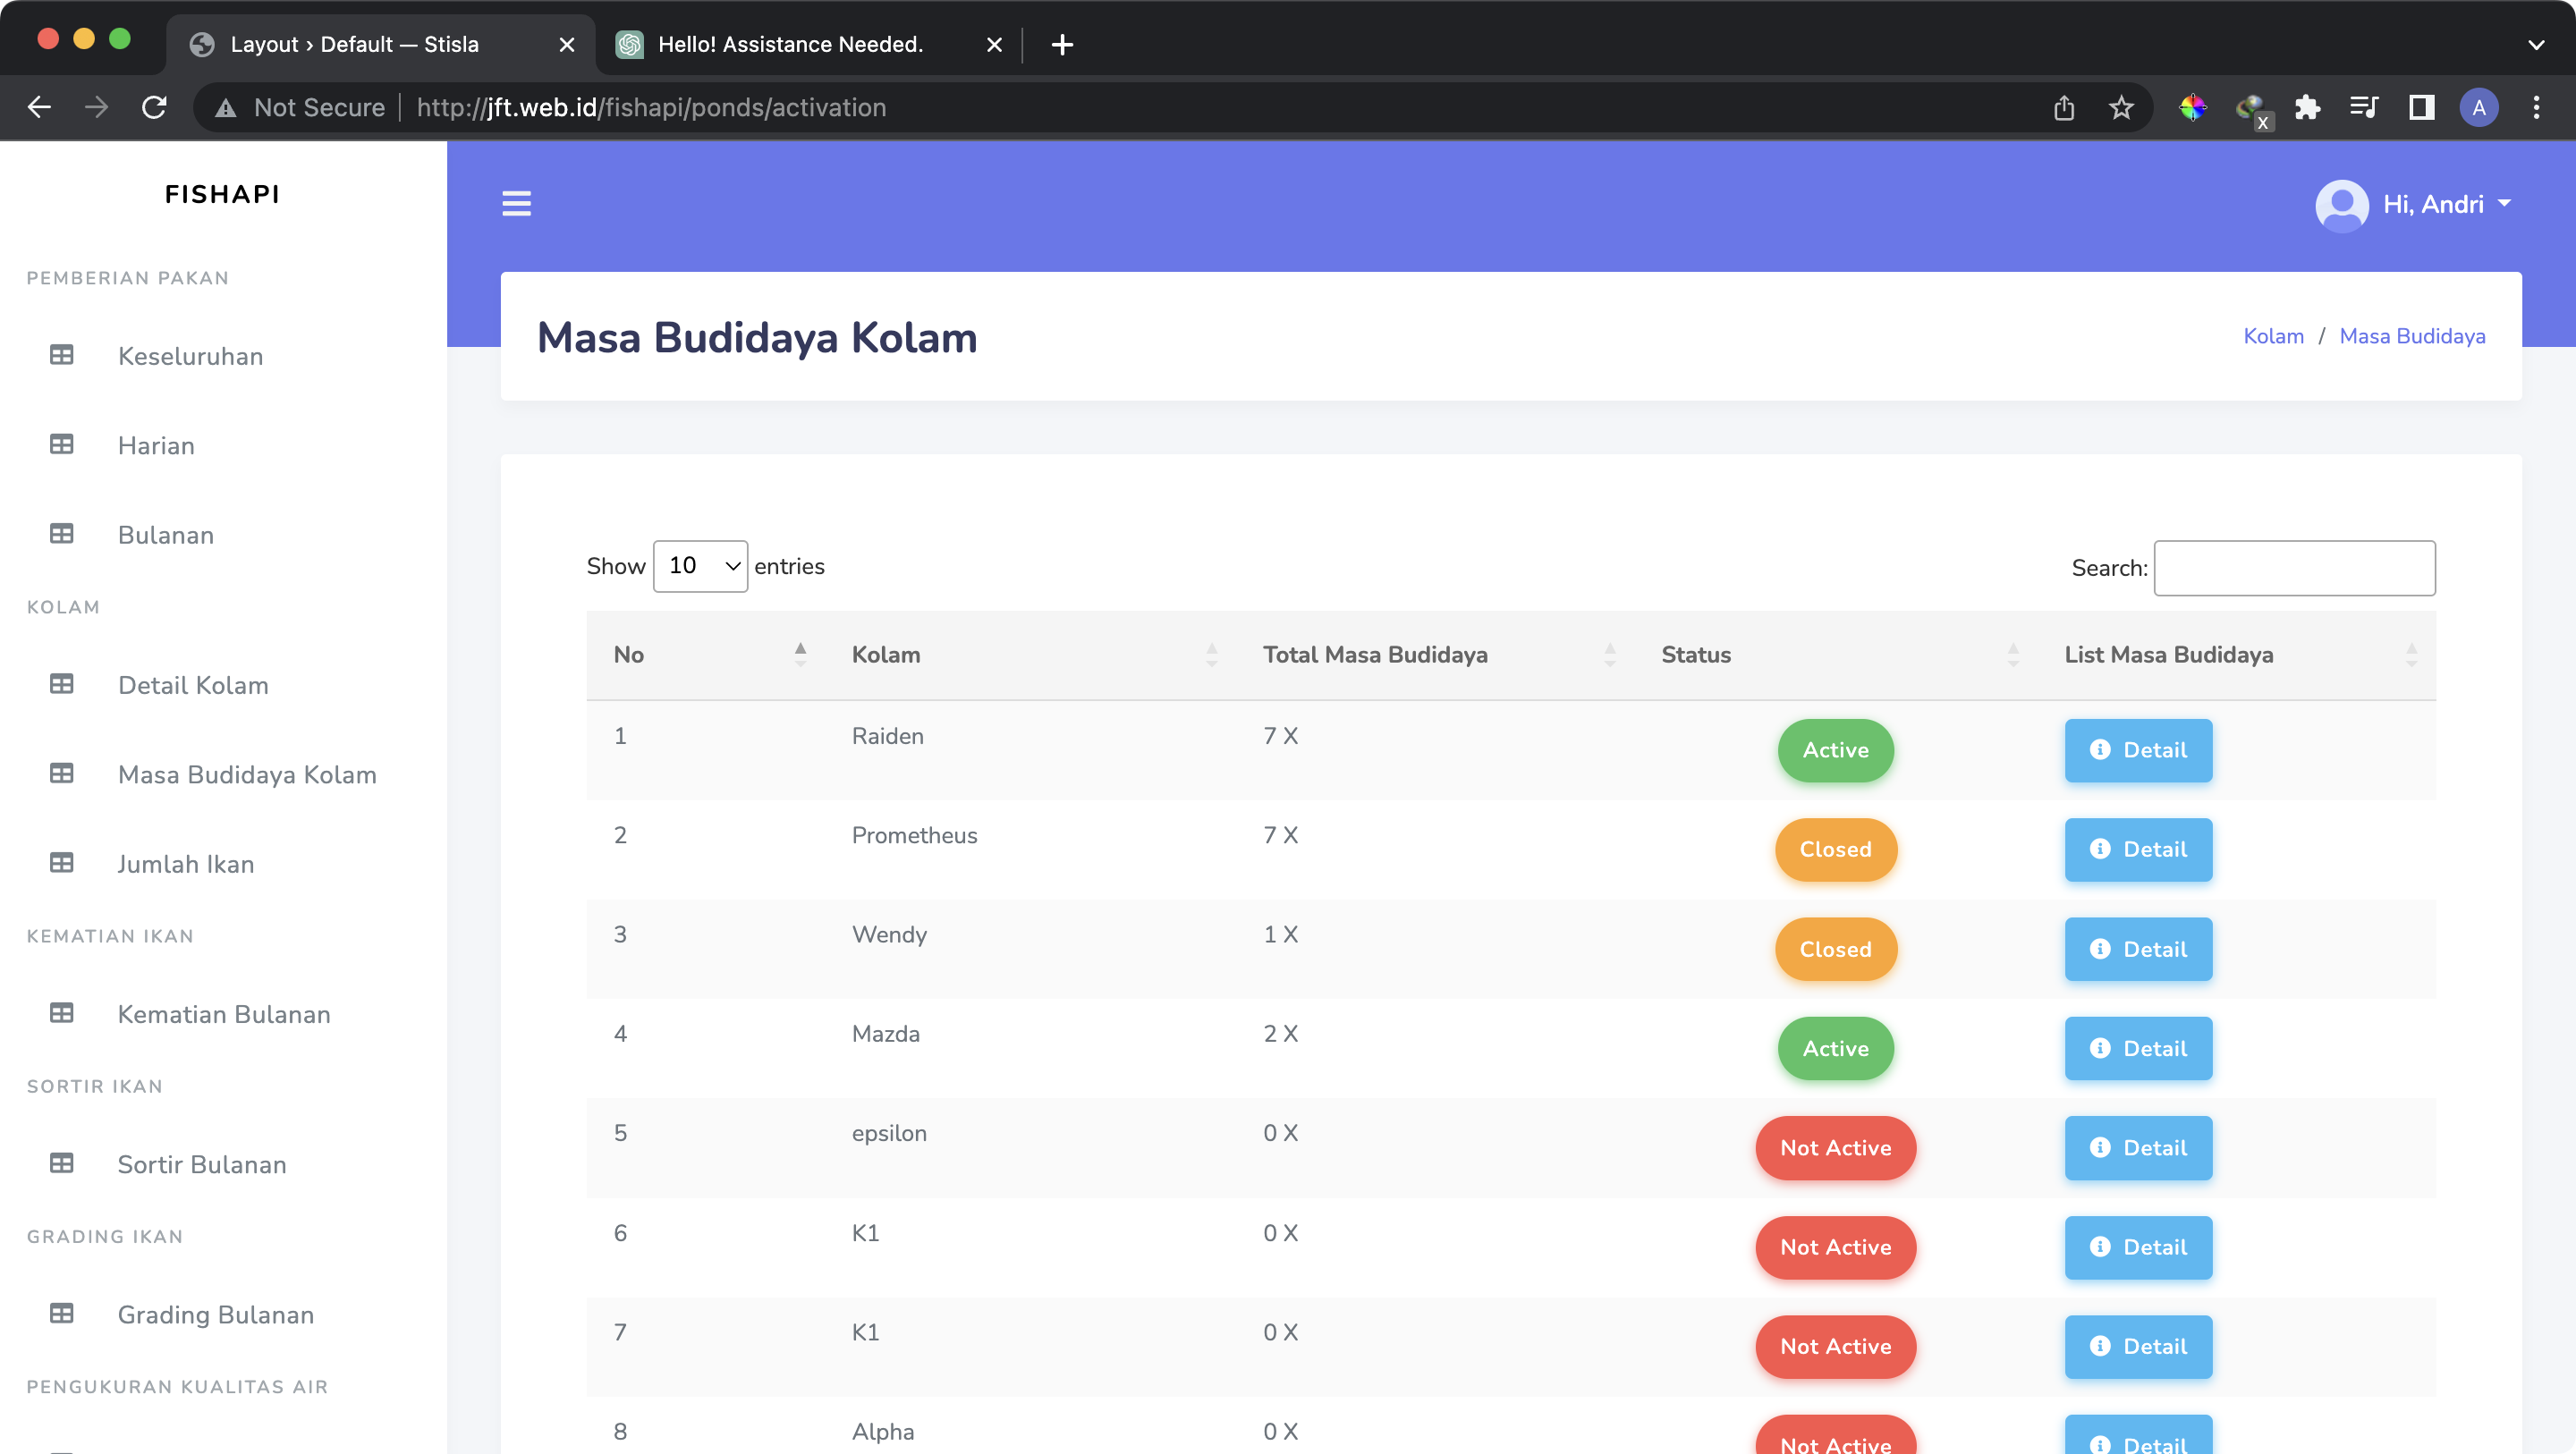
\includegraphics[width=1\textwidth]{gambar/Sprint04/view/view_status_kolam}
	\caption{View status kolam}
	\label{fig:view_status_kolam}
\end{figure}


\item \textbf{Membuat view list budidaya per kolam}
\begin{figure}[H]
	\centering
	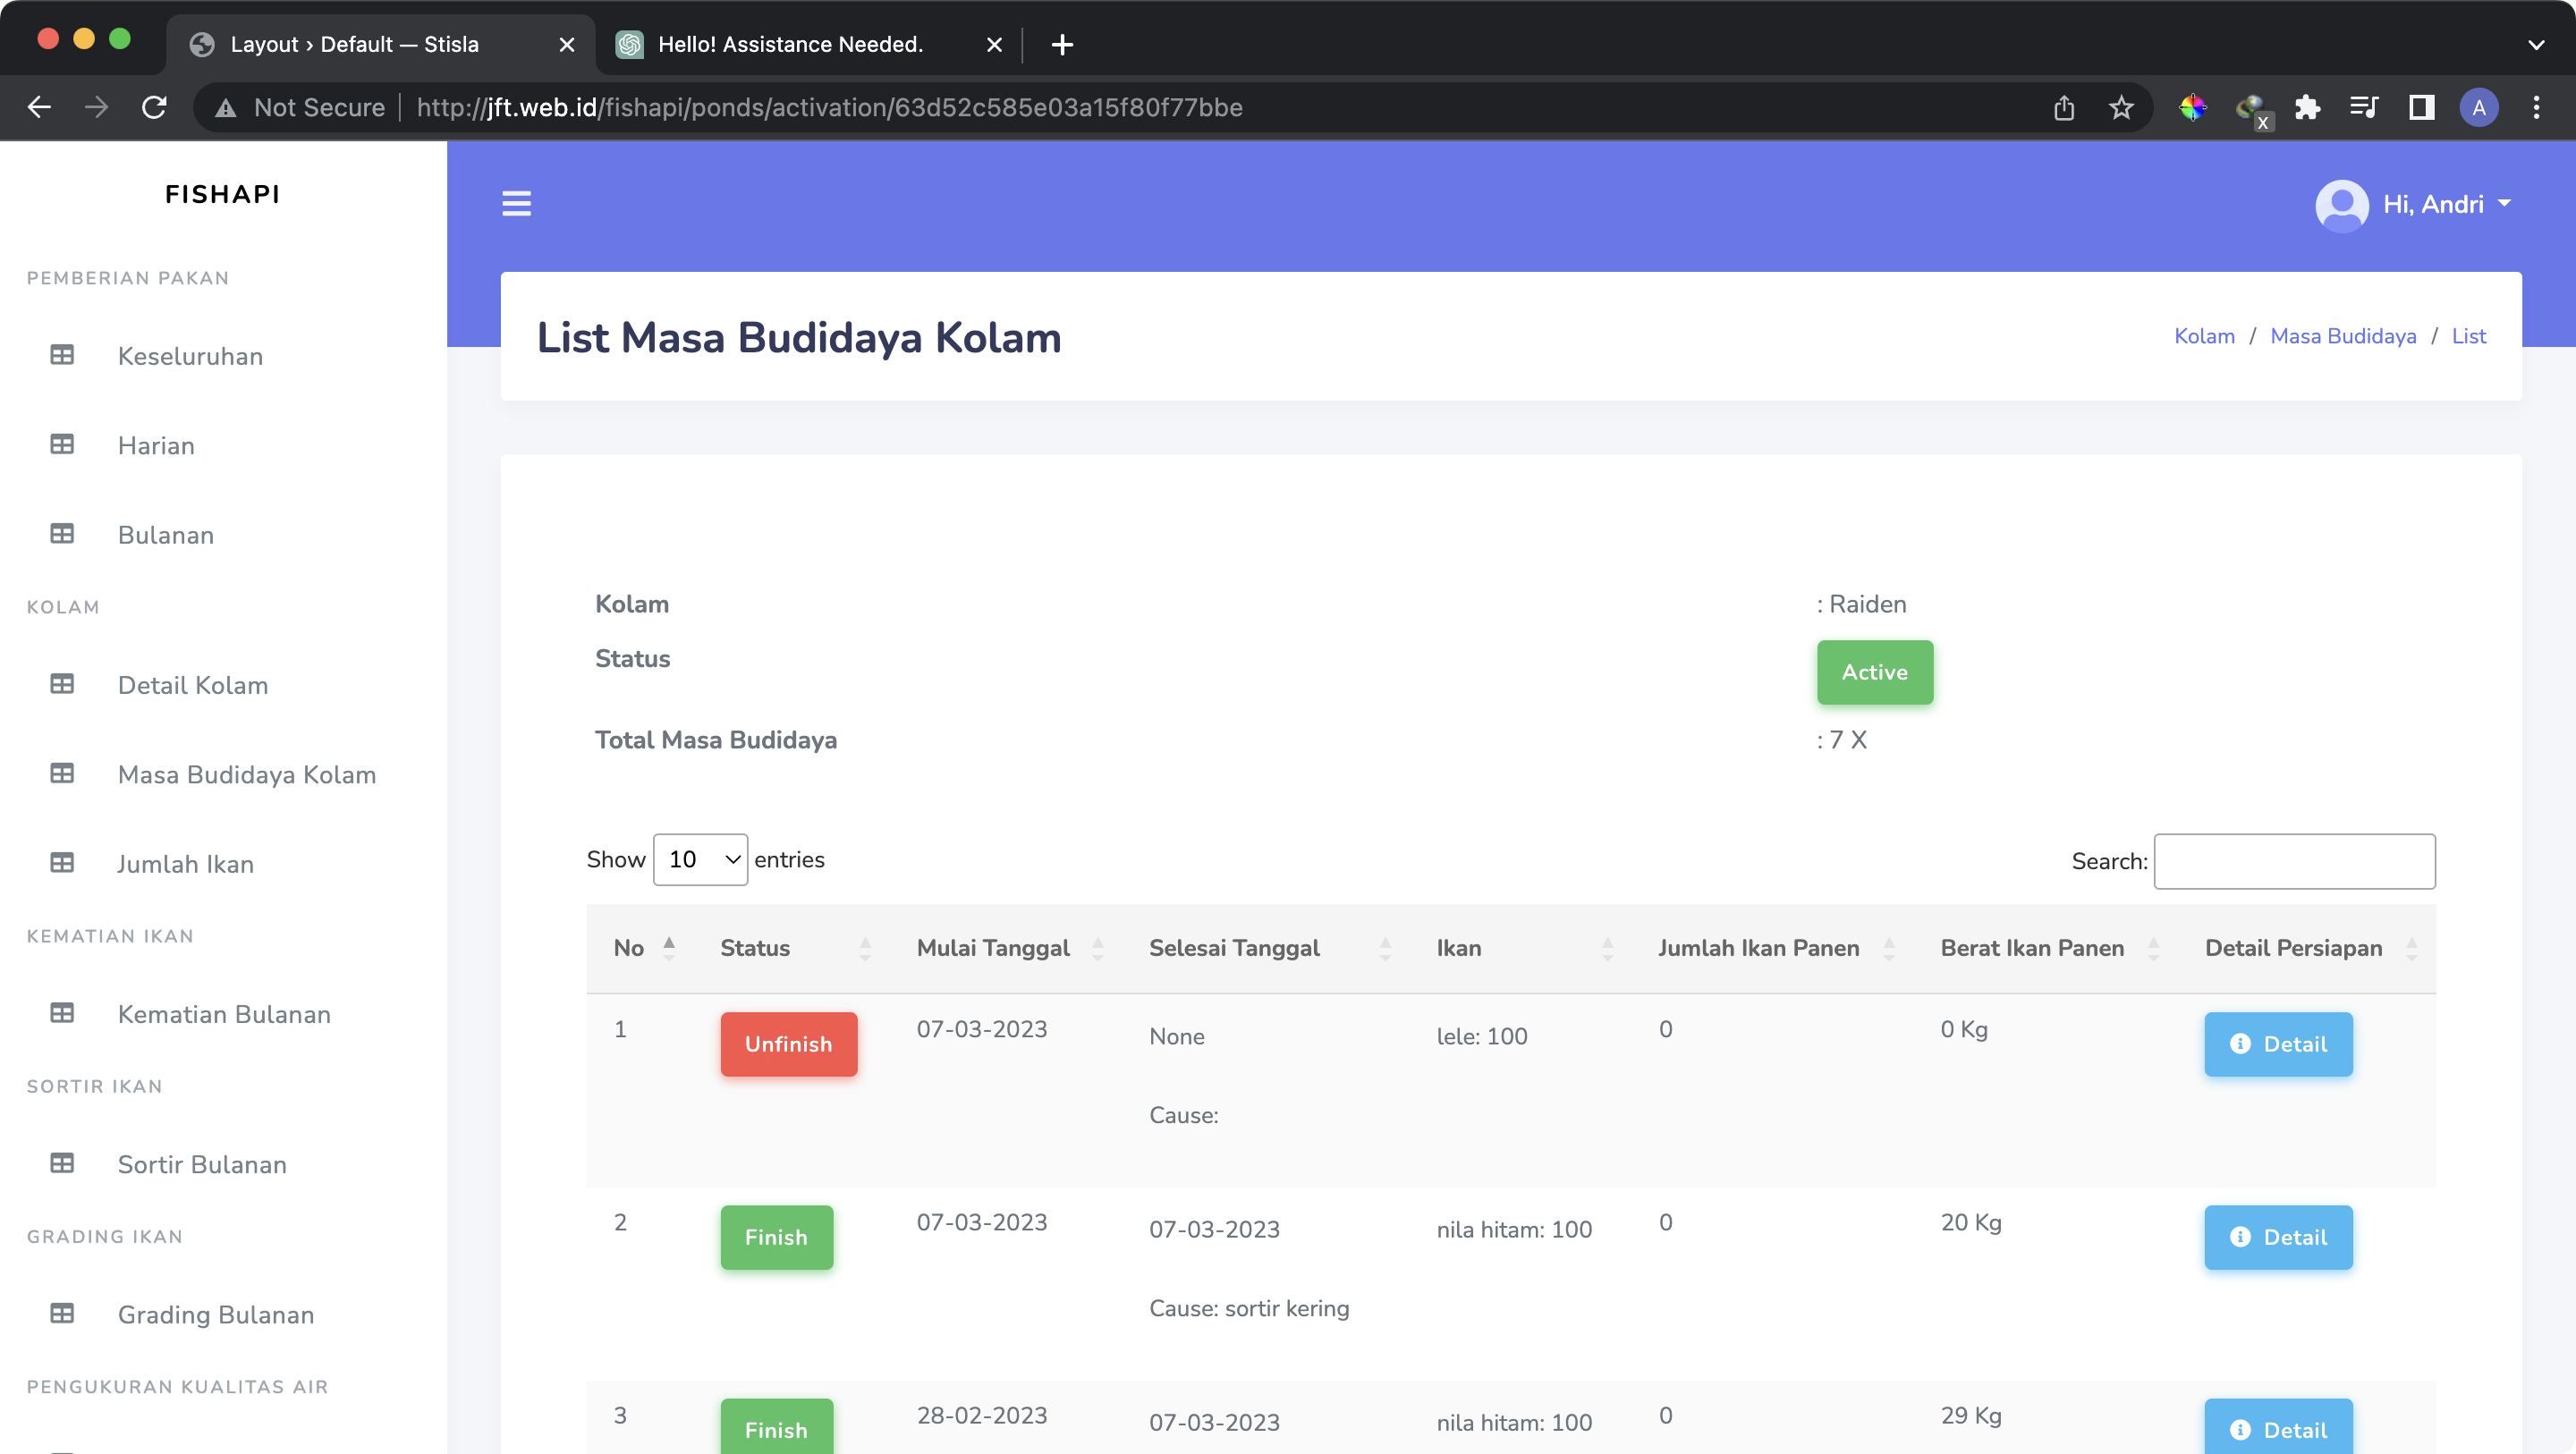
\includegraphics[width=1\textwidth]{gambar/Sprint04/view/view_list_musim_budidaya_perkolam}
	\caption{View list musim budidaya per kolam}
	\label{fig:view_list_musim_budidaya_perkolam}
\end{figure}


\item \textbf{Membuat view detail budidaya}
\begin{figure}[H]
	\centering
	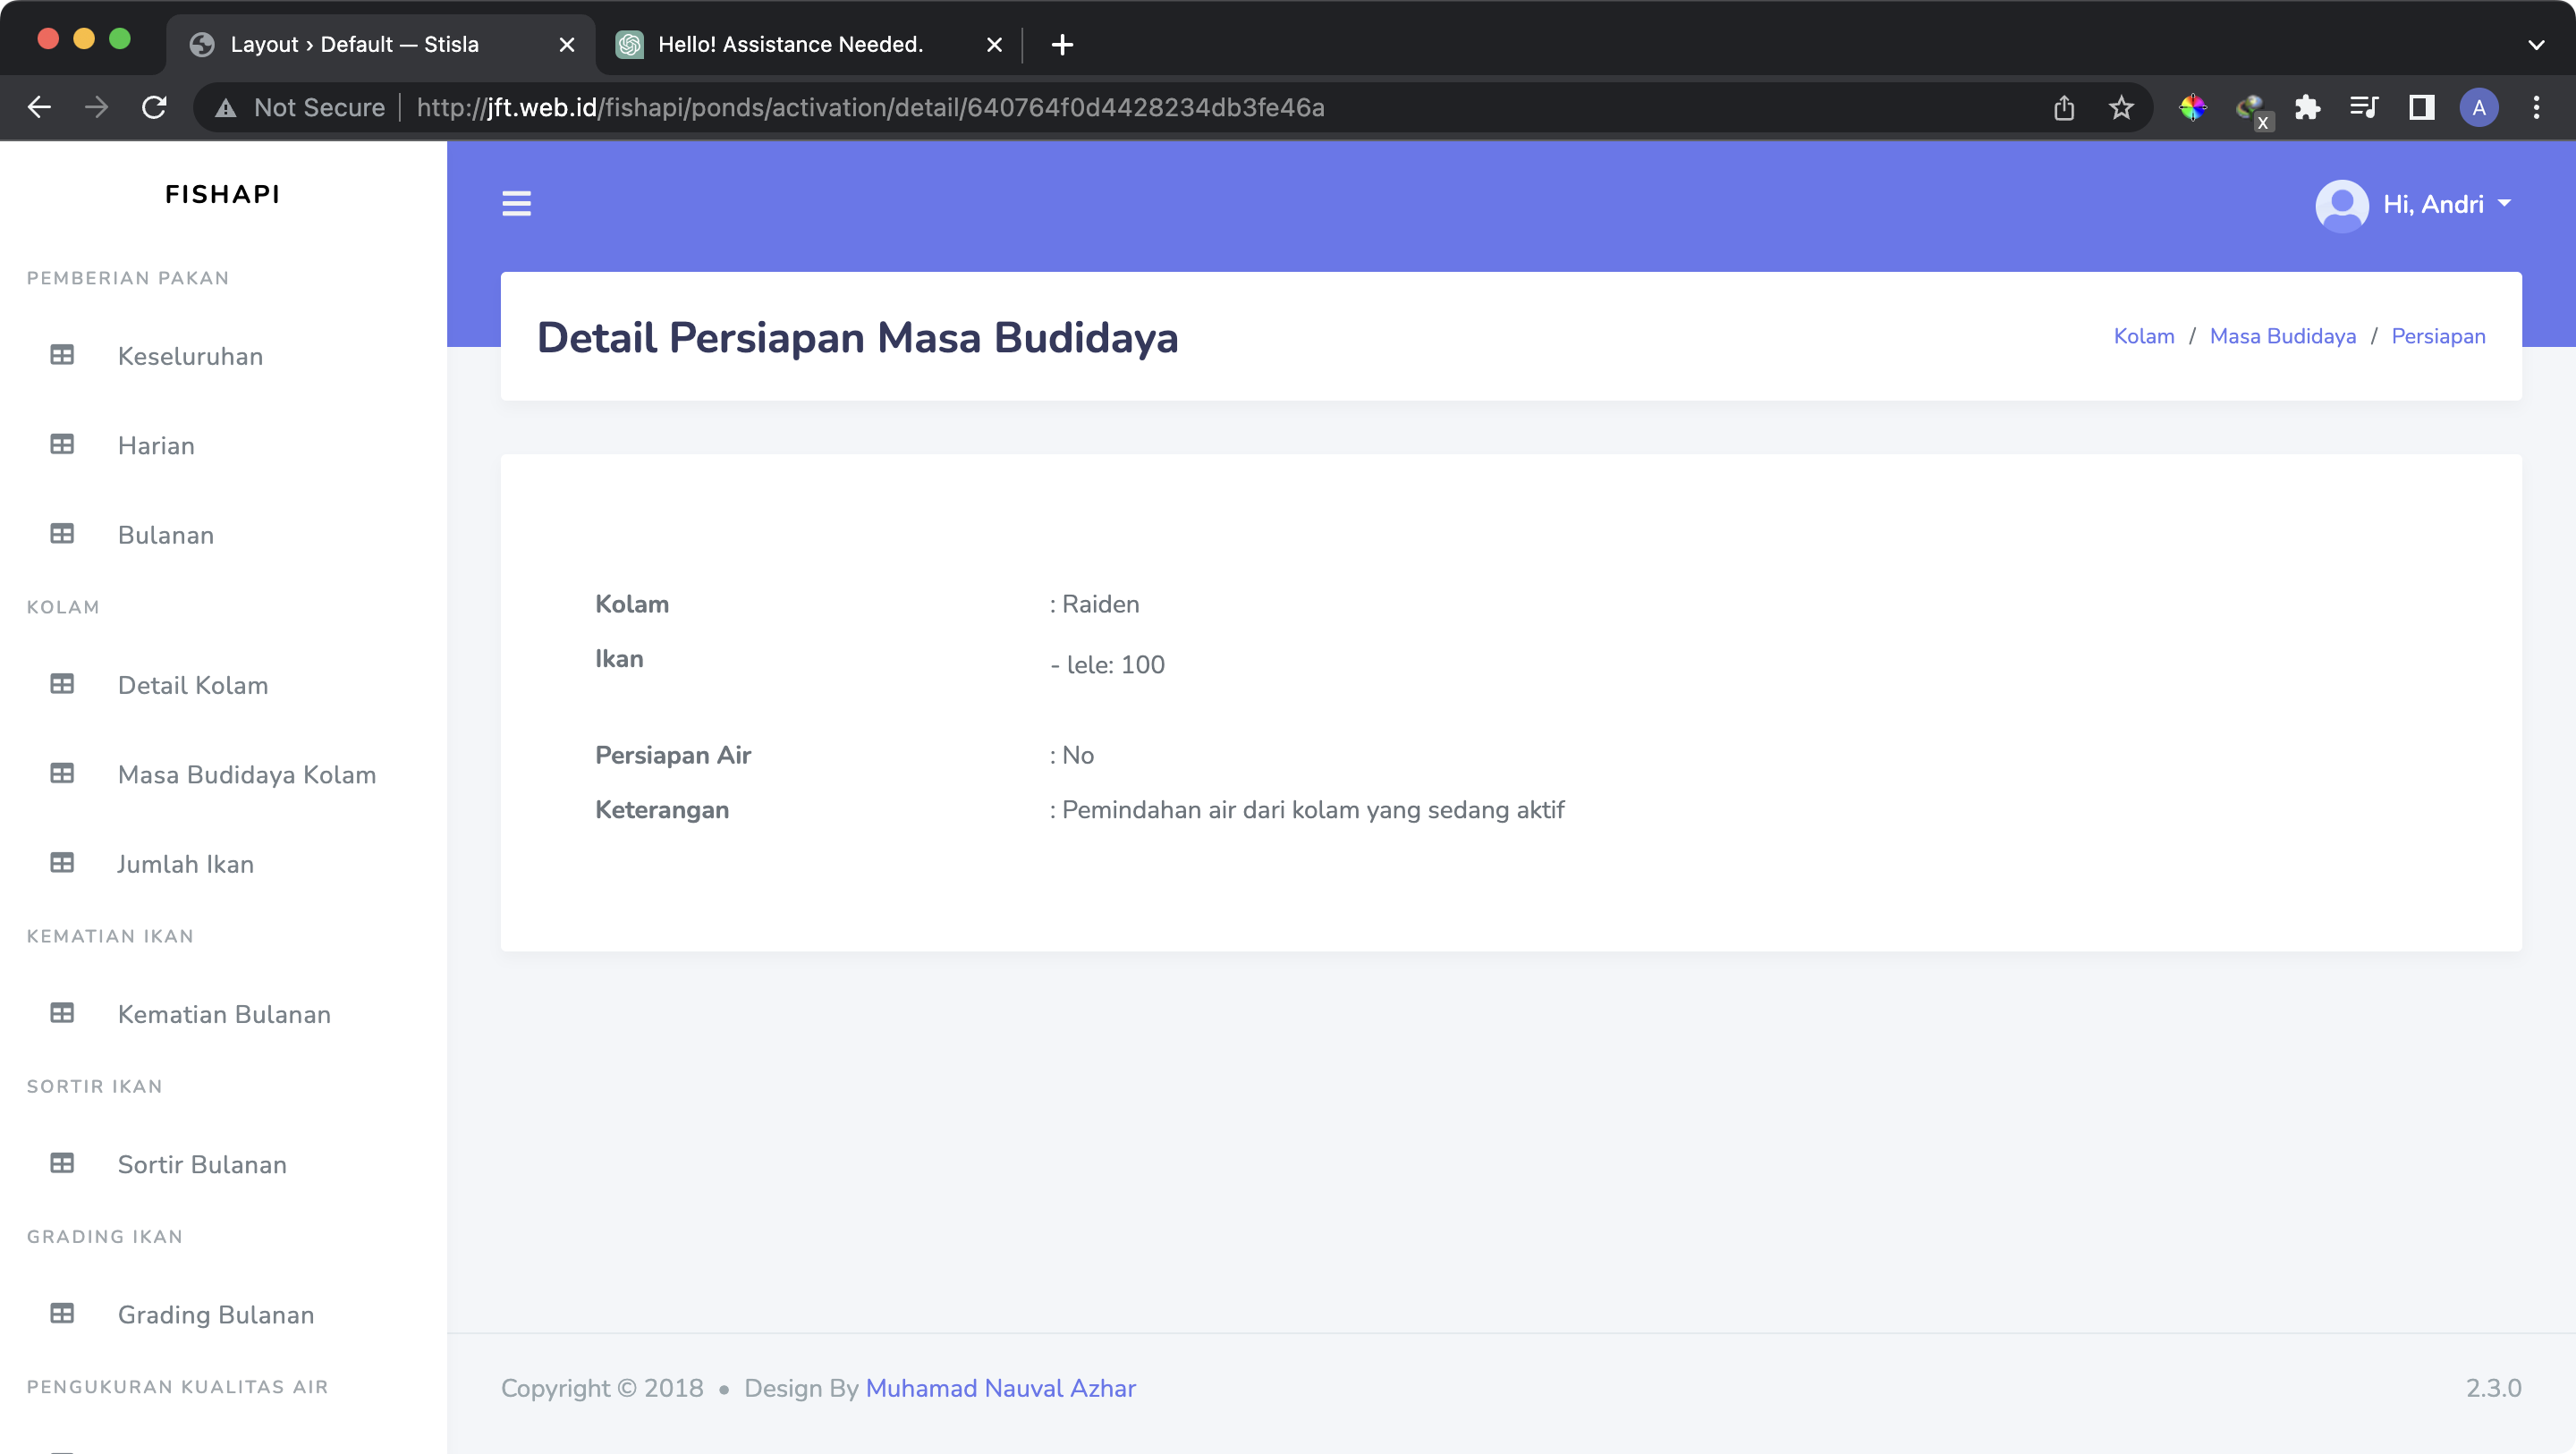
\includegraphics[width=1\textwidth]{gambar/Sprint04/view/view_detail_budidaya}
	\caption{View detail musim budidaya}
	\label{fig:view_detail_budidaya}
\end{figure}



\end{enumerate}